\begin{frame}{\textsc{Часть II}}{Постановка эксперимента}
\begin{columns}
\begin{column}{0.35\textwidth}
\centering
\textbf{СУРА} -- \\
экспериментальный радиокомплекс по воздействию ВЧ излучением на ионосферу. 
\href{https://clck.ru/NfWnc}{Расположен} вблизи Нижнего Новгорода (56,15\degree N, 46,1\degree E). \\ 
Эффективная мощность: 80-240 МВт \\
Диаграмма направленности: карандашной формы шириной 6-12\degree
\end{column}
\begin{column}{0.65\textwidth}
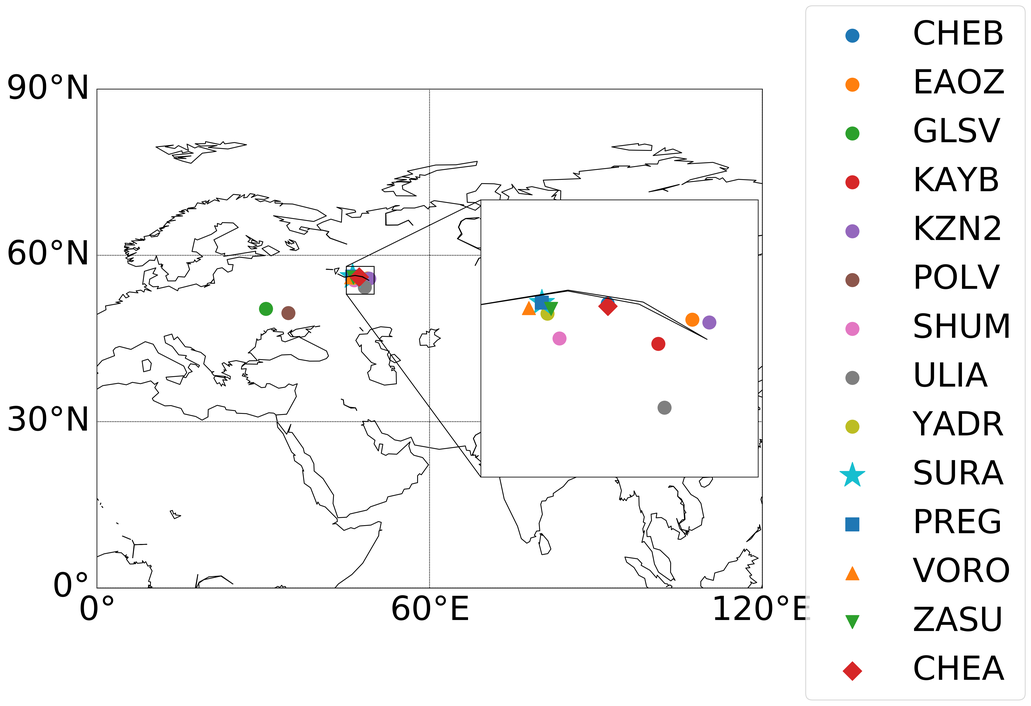
\includegraphics[width=\textwidth]{../fig/sites.png}  
\end{column}
\end{columns}
\end{frame}

\begin{frame}{\textsc{Часть II}}{Режим PPP (23 августа 2010 года)}
\centering
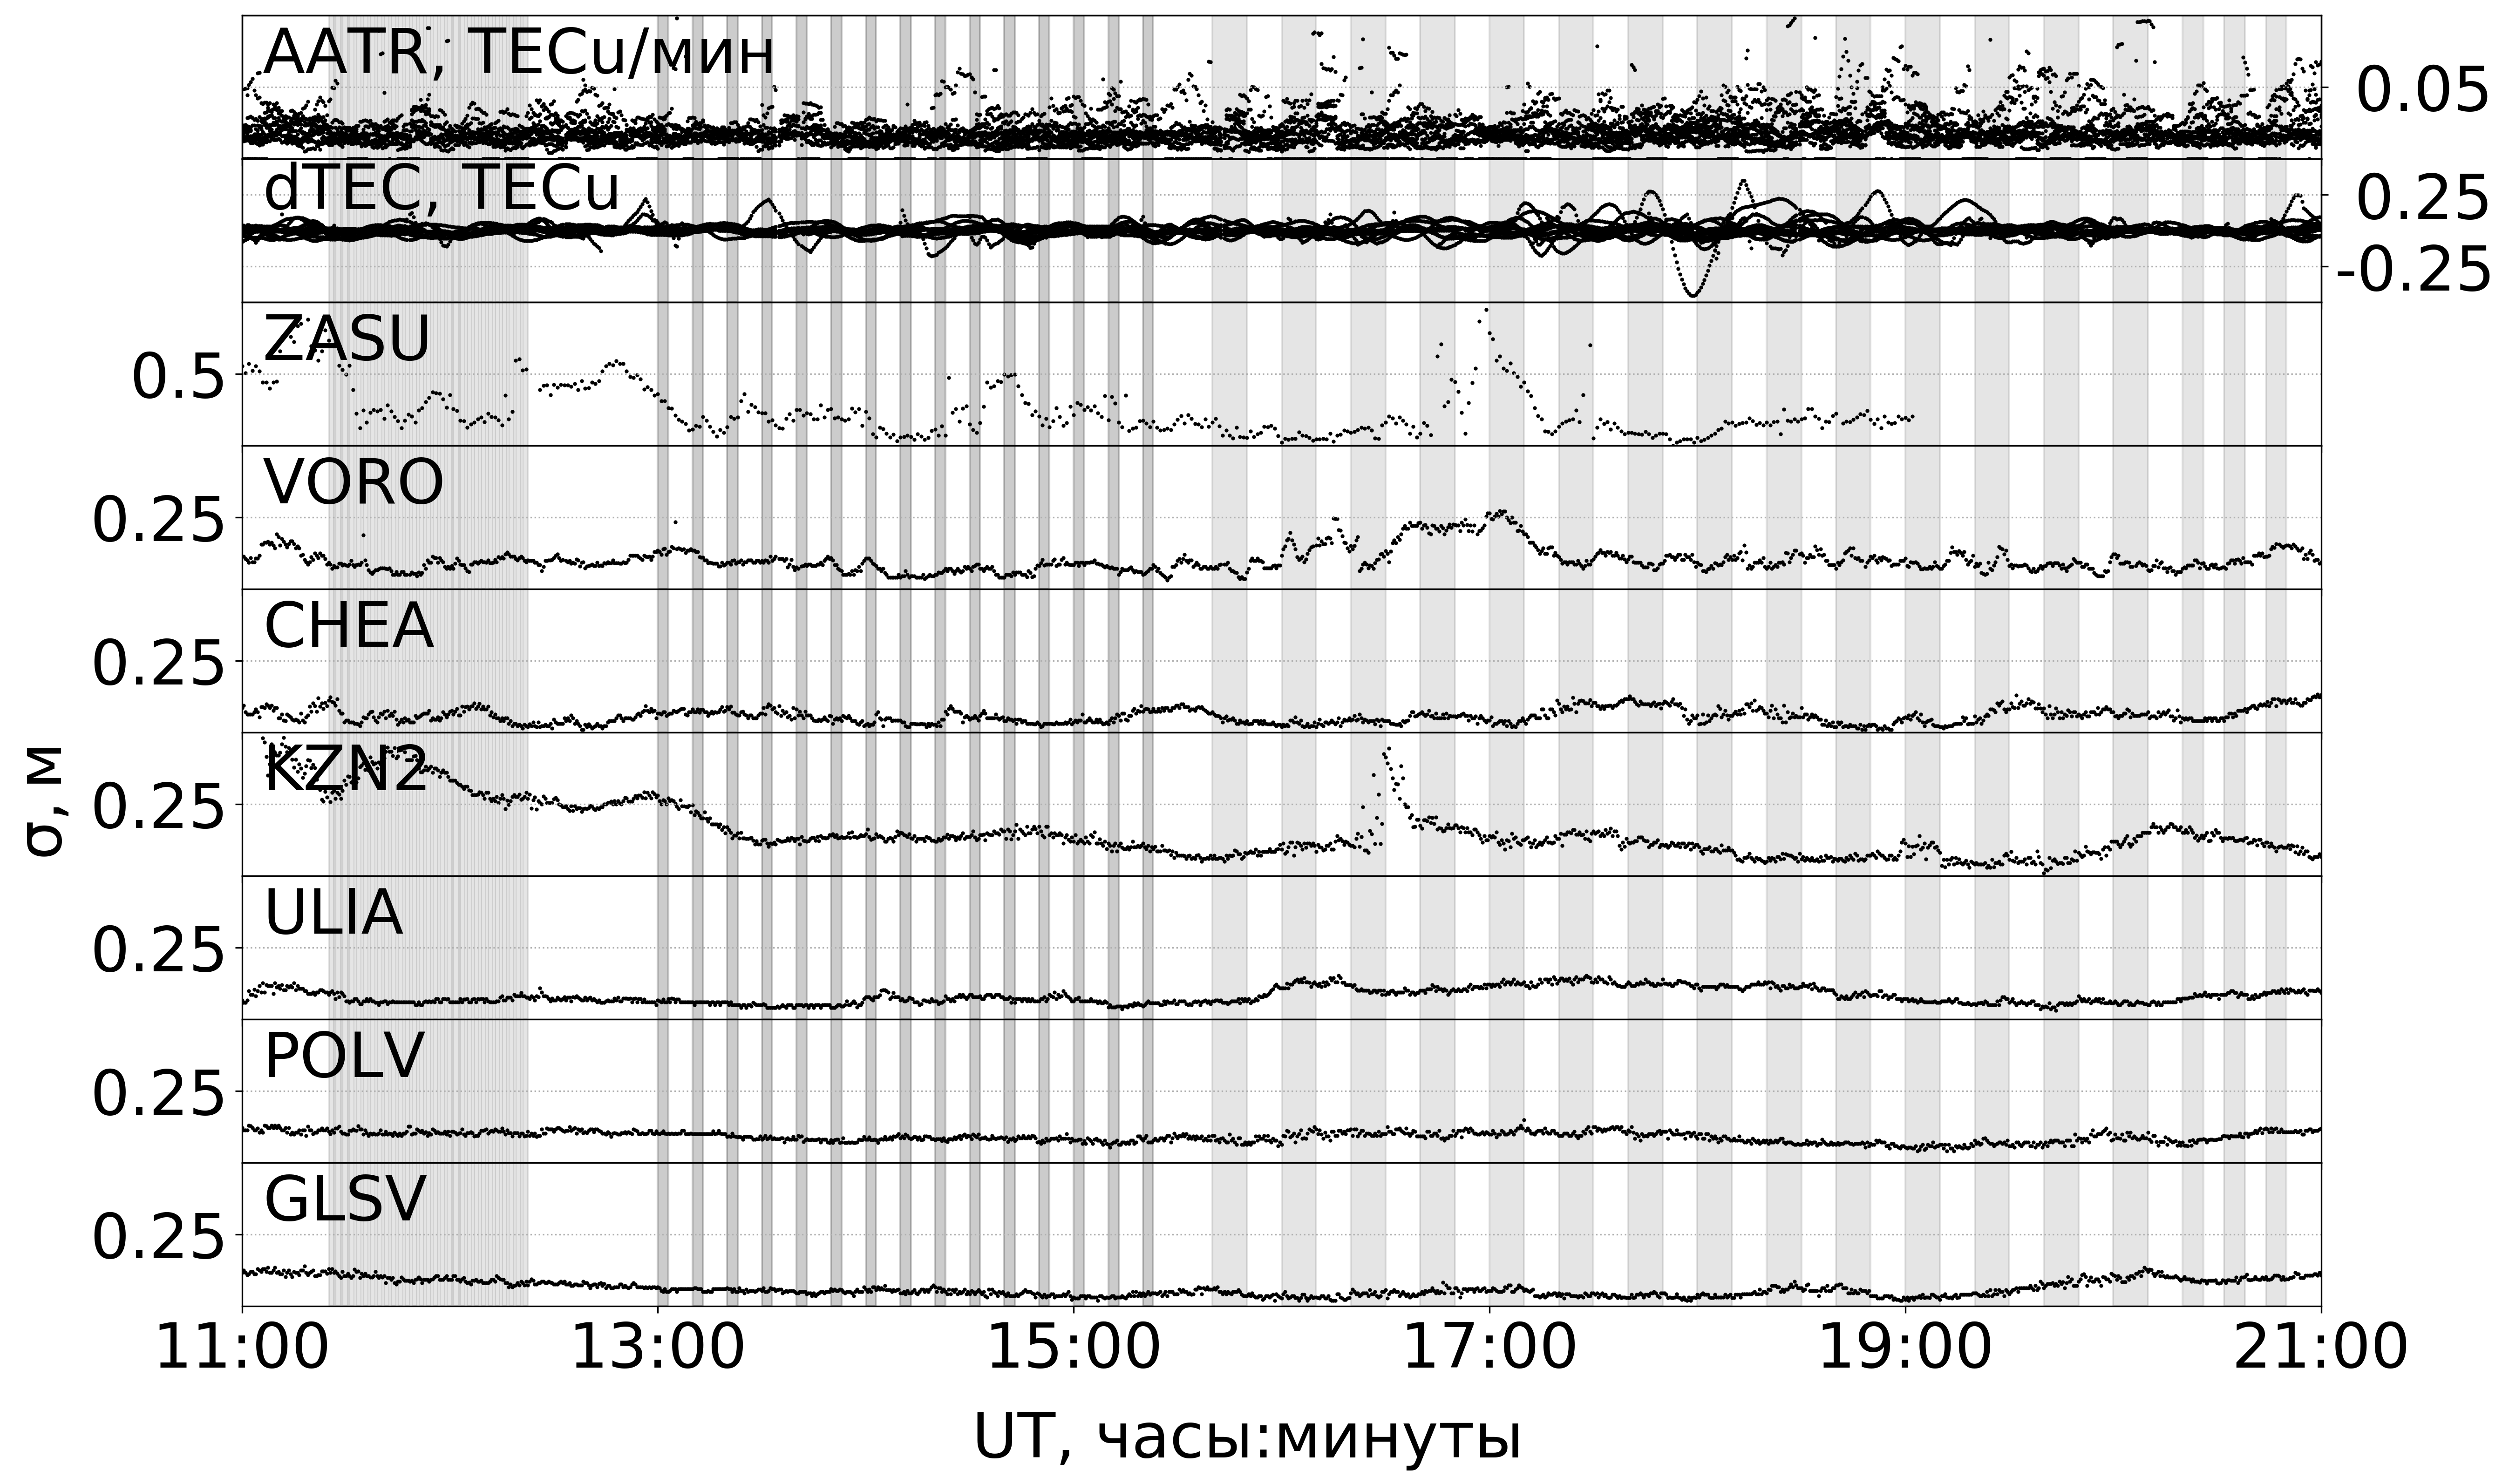
\includegraphics[width=0.9\textwidth]{../fig/src/ppp-2010-235.png}
\end{frame}

\newgeometry{top=0px,bottom=0px,left=-6px,right=0px} 

\begin{landscape}
\begin{frame}
\adjustbox{minipage=\paperheight,padding=-5px 5px 5px 10px,margin=0px 0px 0px 0px,bgcolor=mygrey}{
\begin{flushright}
\color{myred}
{\Large \textsc{Часть II}} \\
{\scriptsize Режим PPP}
\end{flushright}}
\centering
\resizebox{0.95\paperheight}{!}{
\renewcommand{\arraystretch}{1.8}
\begin{tabular}{|>{\centering\arraybackslash}m{4cm}|c|c|}
\hline
Станция & \begin{tabular}[c]{@{}c@{}}$\text{Среднее}\pm\text{СКО}$ ошибки \\ во время нагрева, м\end{tabular} & \begin{tabular}[c]{@{}c@{}}$\text{Среднее}\pm\text{СКО}$ ошибки \\ во время пауз, м\end{tabular} \\ \hline
\multicolumn{3}{|c|}{23 августа 2010 года}                                                                                                                                                                       \\ \hline
ZASU    & $0,27\pm0,56$                                                                                       & $0,36\pm0,70$                                                                                    \\ \hline
VORO    & $0,10\pm0,05$                                                                                       & $0,11\pm0,15$                                                                                    \\ \hline
CHEA    & $0,06\pm0,02$                                                                                       & $0,11\pm0,29$                                                                                    \\ \hline
KZN2    & $0,15\pm0,10$                                                                                       & $0,14\pm0,13$                                                                                    \\ \hline
ULIA    & $0,08\pm0,03$                                                                                       & $0,10\pm0,12$                                                                                    \\ \hline
POLV    & $0,09\pm0,02$                                                                                       & $0,14\pm0,21$                                                                                    \\ \hline
GLSV    & $0,06\pm0,03$                                                                                       & $0,10\pm0,13$                                                                                    \\ \hline
\multicolumn{3}{|c|}{19 сентября 2016 года}                                                                                                                                                                      \\ \hline
SURA    & $0,08\pm0,02$                                                                                       & $0,10\pm0,08$                                                                                    \\ \hline
PREG    & $0,13\pm0,06$                                                                                       & $0,15\pm0,15$                                                                                    \\ \hline
YADR    & $0,07\pm0,03$                                                                                       & $0,12\pm0,12$                                                                                    \\ \hline
CHEB    & $0,07\pm0,03$                                                                                       & $0,11\pm0,09$                                                                                    \\ \hline
SHUM    & $0,09\pm0,03$                                                                                       & $0,12\pm0,10$                                                                                    \\ \hline
KZN2    & $0,39\pm0,43$                                                                                       & $0,21\pm0,29$                                                                                    \\ \hline
POLV    & $0,05\pm0,02$                                                                                       & $0,09\pm0,09$                                                                                    \\ \hline
GLSV    & $0,06\pm0,03$                                                                                       & $0,08\pm0,08$                                                                                    \\ \hline
\multicolumn{3}{|c|}{20 сентября 2016 года}                                                                                                                                                                      \\ \hline
SURA    & $0,11\pm0,04$                                                                                       & $0,15\pm0,10$                                                                                    \\ \hline
PREG    & $0,11\pm0,04$                                                                                       & $0,15\pm0,16$                                                                                    \\ \hline
KAYB    & $0,11\pm0,03$                                                                                       & $0,15\pm0,20$                                                                                    \\ \hline
EAOZ    & $0,11\pm0,03$                                                                                       & $0,12\pm0,12$                                                                                    \\ \hline
KZN2    & $0,10\pm0,03$                                                                                       & $0,13\pm0,17$                                                                                    \\ \hline
POLV    & $0,09\pm0,04$                                                                                       & $0,12\pm0,09$                                                                                    \\ \hline
GLSV    & $0,09\pm0,04$                                                                                       & $0,08\pm0,04$                                                                                    \\ \hline
\end{tabular}}
\end{frame}
\end{landscape}

\newgeometry{top=0px,bottom=5px,left=28px,right=28px} 

\begin{frame}{\textsc{Часть II}}{Результаты\footnote[1]{{\tiny\justifying Ю.В. Ясюкевич, \begin{bf}С.В. Сыроватский\end{bf}, А.М. Падохин, В.Л. Фролов, А.М. Веснин, Д.А. Затолокин, Г.А. Курбатов, Р.В. Загретдинов, А.В. Першин, А.С. Ясюкевич. Точность позиционирования GPS в различных режимах при активном воздействии на ионосферу мощным КВ-излучением нагревного стенда СУРА // Известия вузов. Радиофизика. --- 2020.}}}
\begin{enumerate}
\justifying
\item Рассмотрены три экспериментальных дня работы нагревательного стенда СУРА: за 23 августа 2010 года и 19-20 сентября 2016 года.
\item Эффектов ухудшения точности позиционирования как в режиме PPP, так и в обычном одночастотном режиме \textbf{не обнаружено}.
Возможные причины:
\begin{itemize}
\justifying
\item Область нагрева и амплитуда генерируемых ионосферных возмущений малы $\rightarrow$ количество лучей приёмник-спутник, проходящих через область нагрева, мало $\rightarrow$ статистический вес возможных ошибок при решении навигационной задачи мал $\rightarrow$ снижение итоговой полной ошибки.  
\item Влияние искусственных ПИВ (перемещающихся ионосферных возмущений) на удалённых приёмных станциях замаскировано естественной изменчивостью среднеширотной ионосферы.
\end{itemize}
\end{enumerate}
\end{frame}